%-------------------------------------------------------------------------------
%	PACKAGES AND DOCUMENT CONFIGURATIONS
%-------------------------------------------------------------------------------

\documentclass[titlepage]{article}

\usepackage{listings}
\usepackage[parfill]{parskip} % Creates newline between paragraphs
\usepackage{graphicx} % Required for the inclusion of images
\usepackage{natbib} % Required to change bibliography style to APA
\usepackage{amsmath} % Required for some math elements 

\setlength\parindent{0pt} % Removes all indentation from paragraphs

%\usepackage{times} % Uncomment to use the Times New Roman font

%-------------------------------------------------------------------------------
%	DOCUMENT INFORMATION
%-------------------------------------------------------------------------------

 % Title
\title{Parallel Matrix Multiplication Sum (pmms)\\ OPERATING SYSTEMS ASSIGNMENT}

\author{\textsc{garland,} Christopher (15560955)} % Author name

\date{\today} % Date for the report

\begin{document}

\maketitle % Insert the title, author and date

% If you wish to include an abstract, uncomment the lines below
% \begin{abstract}
% Abstract text
% \end{abstract}

%-------------------------------------------------------------------------------
%	SECTION 1
%-------------------------------------------------------------------------------
\section{ReadMe}

This program will calculate the product of two matrices, and sum the product 
matrix in parallel by using multiple processes/threads. Test files have been 
provided, and will be discussed further in section 3.0.
\par
There is an emphasis on process/thread creation \& synchronization (section 2.0)
and less on  error handling. This means that there are several conditions 
under which the program will not run --- discussed in section 3.0.
\par
This project should compile and run on any of the lab machines. 
\texttt{gdb} was used to test the program. Where possible \texttt{valgrind} 
has been used to check for memory leaks. Further discussion of testing in 
section 3.0.

\subsection{Instructions for Compilation}
\begin{itemize}
	\item Compile all binary files and report: \texttt{make}
    \item Compile only binary files: \hspace{37pt} \texttt{make bin}
    \item Compile only report: \hspace{58pt} \texttt{make report}
    \item Delete all generated files: \hspace{39pt} \texttt{make clean}
\end{itemize}

\subsection{Instructions for Execution}
Included within this project are eight matrix description files that can be 
provided as arguments to the programs. The files (along with their 
dimensions) are to be used as program arguments in the following 4 pairs.
\begin{enumerate}
	\item \texttt{description-A description-B 3 2 4}
	\item \texttt{description-C description-D 3 3 3}
	\item \texttt{description-E description-F 3 5 4}
	\item \texttt{description-G description-H 5 2 5}
\end{enumerate}
For the purpose of these instructions, pair 1 will be used. The programs can be
executed as follows.
\begin{itemize}
	\item Processes: 
    	\texttt{./pmms-process description-A description-B 3 2 4}
    \item Threads: 
    	\hspace{6pt}\texttt{./pmms-thread description-A description-B 3 2 4}
    \item Both: 
    	\hspace{20pt}\texttt{./pmms description-A description-B 3 2 4}
\end{itemize}

%-------------------------------------------------------------------------------
%	SECTION 2
%-------------------------------------------------------------------------------
\section{Mutual Exclusion \& Synchronization}

Mutual exclusion and process/thread synchronization is achieved with the use 
of mutex locks and semaphores. In both cases (processes \& threads), we are 
faced with the producer/consumer problem and have a bounded buffer with a 
size of 1.

\subsection{Using Processes}
The main strategies to achieve process synchronization were to use shared 
memory blocks and semaphores. Source can be found in \texttt{process-control.c}
\par
A semaphore struct was created and used. The source code can be viewed in 
the file \texttt{semaphore.h}. The struct contains a \texttt{mutex} 
variable that is used as a binary lock, and is initialized to 0. There are 
two other  variables \texttt{empty} and \texttt{full}. As the buffer is only 
of size 1, these variables are binary in nature, and are initialized to 1 and 
0 respectively. 
\par
The tactic employed is further illustrated in Figure 1.

\begin{figure}[ht]
\begin{center}
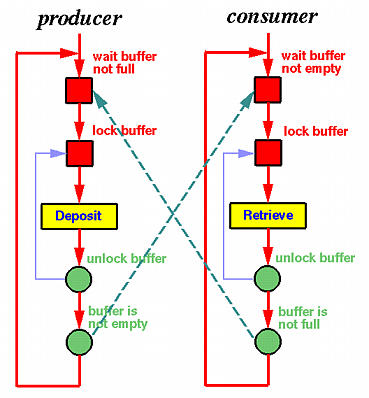
\includegraphics[width=0.65\textwidth]{Prod-Cons} % Include the image 
													% Prod-Cons.png
\caption{Producer/Consumer with bounded buffer.}
\end{center}
\end{figure}

\subsection{Using Threads}
Mutex lock with condition variables were used to achieve mutual exclusion. No 
shared memory blocks were created as threads already share memory with the 
parent. 
\par
Source code can be found in \texttt{thread-control.c}
 
%-------------------------------------------------------------------------------
%	SECTION 3
%-------------------------------------------------------------------------------
\section{Known Faults \& Testing}
The focus for this assignment was on process/thread creation and 
synchronization and less on error handling. This means there are conditions 
upon which this program will not run. 

\subsection{Input Files \& Error Handling}
The program truncates the first 2 lines 
of a file before reading in the matrix values. This is by no means the best 
way to implement a file read but as it stands, there are very strict rules for 
input files...

\begin{itemize}
	\item Files must have exactly two lines (of anything) before the matrix 
    values
    \item The number of matrix values in the files MUST match the dimensions 
    	  provided.
\end{itemize}

\clearpage

\subsection{Memory Leaks}
There are known memory leaks. Here is a \texttt{valgrind} leak check:

\begin{lstlisting}
==30966== 
==30966== HEAP SUMMARY:
==30966==     in use at exit: 1,789 bytes in 27 blocks
==30966==   total heap usage: 29 allocs, 2 frees, 2,301 bytes allocated
==30966== 
==30966== LEAK SUMMARY:
==30966==    definitely lost: 788 bytes in 5 blocks
==30966==    indirectly lost: 0 bytes in 0 blocks
==30966==      possibly lost: 0 bytes in 0 blocks
==30966==    still reachable: 1,001 bytes in 22 blocks
==30966==         suppressed: 0 bytes in 0 blocks
==30966== Rerun with --leak-check=full to see details of leaked memory
==30966== 
==30966== For counts of detected and suppressed errors, rerun with: -v
==30966== ERROR SUMMARY: 0 errors from 0 contexts (suppressed: 14 from 8)
==30967== 
==30967== HEAP SUMMARY:
==30967==     in use at exit: 1,789 bytes in 27 blocks
==30967==   total heap usage: 29 allocs, 2 frees, 2,301 bytes allocated
==30967== 
==30967== LEAK SUMMARY:
==30967==    definitely lost: 788 bytes in 5 blocks
==30967==    indirectly lost: 0 bytes in 0 blocks
==30967==      possibly lost: 0 bytes in 0 blocks
==30967==    still reachable: 1,001 bytes in 22 blocks
==30967==         suppressed: 0 bytes in 0 blocks
==30967== Rerun with --leak-check=full to see details of leaked memory
==30967== 
==30967== For counts of detected and suppressed errors, rerun with: -v
==30967== ERROR SUMMARY: 0 errors from 0 contexts (suppressed: 14 from 8)
Subtotal produced by thread with ID 81902448: 62
Subtotal produced by thread with ID 92392304: 134
Subtotal produced by thread with ID 102882160: 206
Total: 402
\end{lstlisting}

\clearpage

%-------------------------------------------------------------------------------
%	SECTION 4
%-------------------------------------------------------------------------------

\section{Example I/O}
In addition to the required output, this program outputs a system call to 
\texttt{ps} to a file called \texttt{psout}. This is to prove the existence of
the running processes. Here is an example of  \texttt{psout} after running the 
program...
\begin{lstlisting}
  PID TTY           TIME CMD
 1089 ttys001    0:00.67 -zsh
 2896 ttys001    0:00.00 ./pmms description-A description-B 3 2 4
 2897 ttys001    0:00.00 (pmms)
 2898 ttys001    0:00.00 ./pmms description-A description-B 3 2 4
 2899 ttys001    0:00.00 ./pmms description-A description-B 3 2 4
 2900 ttys001    0:00.00 sh -c ps > psout
\end{lstlisting}

We can clearly see that there were 4 processes created. This is the expected 
result given the following test input.

\subsection{Input}
Example of first input file:
\begin{lstlisting}
# Matrix A: 3 x 2

1 2
3 4
5 6
# EOF
\end{lstlisting}

Example of second input file:
\begin{lstlisting}
# Matrix B: 2 x 4

1 2 3 4
5 6 7 8

# EOF
\end{lstlisting}
\subsection{Output}
When run with \texttt{./pmms-process description-A description-B 3 2 4}
\begin{lstlisting}
Subtotal produced by process with ID 2897: 62
Subtotal produced by process with ID 2898: 134
Subtotal produced by process with ID 2899: 206
Total: 402
\end{lstlisting}
When run with \texttt{./pmms-thread description-A description-B 3 2 4}
\begin{lstlisting}
Subtotal produced by thread with ID 87359488: 62
Subtotal produced by thread with ID 87896064: 134
Subtotal produced by thread with ID 88432640: 206
Total: 402
\end{lstlisting}
When run with \texttt{./pmms description-A description-B 3 2 4}
\begin{lstlisting}
Subtotal produced by process with ID 2897: 62
Subtotal produced by process with ID 2898: 134
Subtotal produced by process with ID 2899: 206
Total: 402

Subtotal produced by thread with ID 87359488: 62
Subtotal produced by thread with ID 87896064: 134
Subtotal produced by thread with ID 88432640: 206
Total: 402
\end{lstlisting}
\end{document}












